\chapter{Syntheseplanning en groene chemie}\label{ch:g12:synthesis-strategy}

Dezelfde pijnstiller, ibuprofen, is op twee manieren gemaakt. De oudere
route telt zes stappen, en van elke honderd kilogram uitgangsstoffen die
ze inkoopt, eindigt zestig kilogram als afval. De nieuwere telt drie
stappen, en houdt bijna elk \omterm{def:g7:atoms-and-molecules:atom}{atoom} dat ze inkoopt. Allebei leveren ze
hetzelfde witte poeder in de tablet; ze verschillen in de planning. Een
scheikundige die een \omterm{def:g10:synthesis-yield:synthesis}{synthese} plant, stelt vier vragen: hoe gaat het
snel, hoe krijg je veel, hoe raak je alleen het juiste deel van een
\omterm{def:g7:atoms-and-molecules:molecule}{molecuul}, en hoe verspil je weinig?

\begin{recall}
Een \omterm{def:g10:synthesis-yield:synthesis}{synthese}: reactie, scheiding, zuivering, identificatie; haar
\omterm{def:g10:synthesis-yield:yield}{rendement} (\cref{ch:g10:synthesis-yield}). \omterm{def:g12:curly-arrows:curly-arrow}{Gebogen pijlen}, substitutie,
additie, \omterm{def:g12:curly-arrows:categories}{eliminatie} (\cref{ch:g12:curly-arrows}). Een \omterm{def:g12:catalysis:catalyst}{katalysator} versnelt
een reactie zonder verbruikt te worden (\cref{ch:g12:catalysis}). Een
\omterm{def:g12:equilibrium:non-total}{niet-aflopende reactie} stopt bij $Q = K$; een overmaat van een \omterm{def:g7:chemical-reactions:reactant}{beginstof},
of het weghalen van een \omterm{def:g7:chemical-reactions:reactant}{reactieproduct}, brengt haar verder
(\cref{ch:g12:equilibrium}).
\end{recall}

\begin{omfigure}
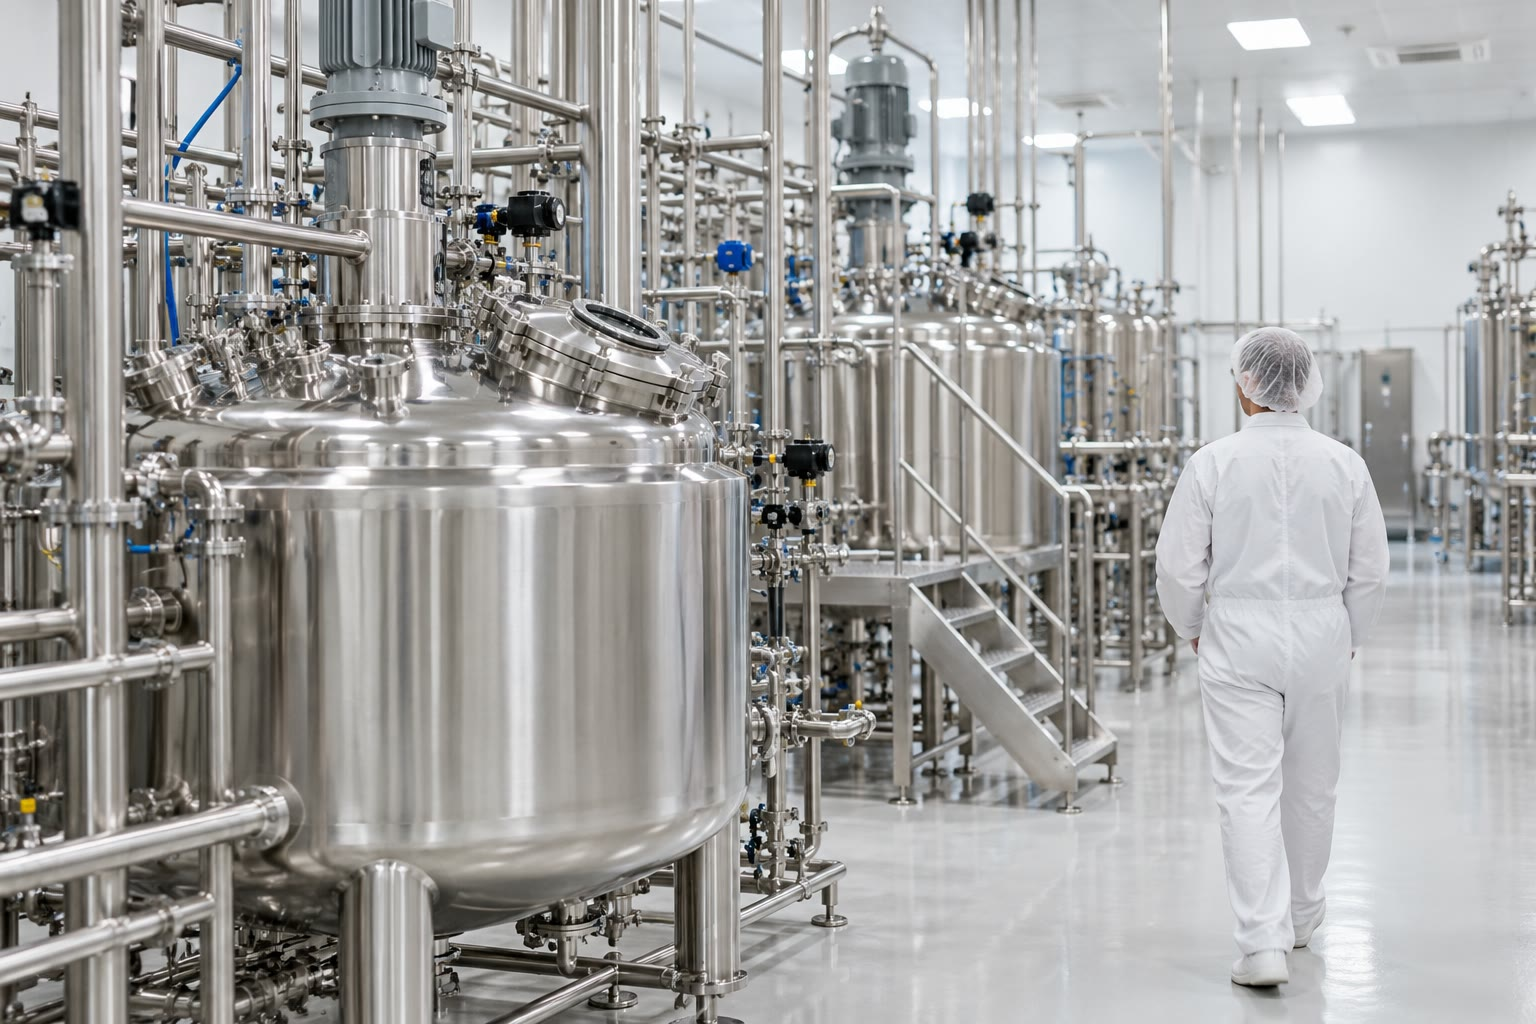
\includegraphics[width=0.48\linewidth]{images/book1/ai/g12-pharma-plant.jpg}

{\small Een farmaceutische fabriek: de reactoren van een \omterm{def:g10:synthesis-yield:synthesis}{synthese},
opgeschaald tot tonnen.}
\end{omfigure}

\section{Een synthese optimaliseren}

Twee verschillende dingen kun je verbeteren: de \emph{snelheid}, die
bepaalt hoe lang de \omterm{def:g10:synthesis-yield:synthesis}{synthese} duurt, en het \emph{\omterm{def:g10:synthesis-yield:yield}{rendement}}, dat bepaalt
hoeveel product ze oplevert.

\begin{proposition}[Knoppen voor snelheid en rendement]\label{prop:g12:synthesis-strategy:levers}
\begin{itemize}
  \item De snelheid neemt toe met de temperatuur, met de concentraties
        van de \omterm{def:g7:chemical-reactions:reactant}{beginstoffen}, en met een \omterm{def:g12:catalysis:catalyst}{katalysator}.
  \item Het eindrendement van een \omterm{def:g10:reaction-progress-table:limiting}{aflopende reactie} ligt vast door de
        \omterm{def:g10:reaction-progress-table:limiting}{beperkende beginstof}; dat van een \omterm{def:g12:equilibrium:non-total}{niet-aflopende reactie} neemt toe
        met een overmaat van een \omterm{def:g7:chemical-reactions:reactant}{beginstof}, of door een \omterm{def:g7:chemical-reactions:reactant}{reactieproduct} weg
        te halen zodra het ontstaat. Een \omterm{def:g12:catalysis:catalyst}{katalysator} verandert het niet:
        hij brengt het systeem alleen sneller naar dezelfde \omterm{def:g10:reaction-progress-table:system}{eindtoestand}.
\end{itemize}
\end{proposition}

\begin{proof}
Het eerste punt verzamelt de \omterm{def:g12:reaction-rates:kinetic-factor}{kinetische factoren} van
\cref{ch:g12:reaction-rates,ch:g12:catalysis}. Het tweede volgt uit
$Q = K$ aan het eind van een \omterm{def:g12:equilibrium:non-total}{niet-aflopende reactie}: een \omterm{def:g7:chemical-reactions:reactant}{beginstof}
toevoegen of een \omterm{def:g7:chemical-reactions:reactant}{reactieproduct} weghalen maakt $Q < K$, en de reactie gaat
verder in de heengaande richting.
\end{proof}

\begin{example}[Verestering met een waterafscheider]\label{ex:g12:synthesis-strategy:trap}
Ethaanzuur en ethanol, één \omterm{def:g10:the-mole:amount}{mol} van elk, geven in evenwicht maar
\qty{67}{\percent} \omterm{def:g11:functional-groups:carboxylic-acid}{ester}. Als het \omterm{def:g6:pure-substances-and-mixtures:mixture}{mengsel} onder terugvloeiing verwarmd
wordt in een \omterm{def:g6:solutions-and-solubility:solute}{oplosmiddel} dat niet met water \omterm{def:g2:mixing-and-dissolving:mix}{mengt}, met een beetje zuur
als \omterm{def:g12:catalysis:catalyst}{katalysator}, condenseert de damp in een zijbuis, een
\emph{waterafscheider}: het water, dat een grotere dichtheid heeft, zakt
naar de bodem en blijft daar, terwijl het \omterm{def:g6:solutions-and-solubility:solute}{oplosmiddel} terugstroomt in de
kolf. Water verlaat de reactie zodra het ontstaat, $Q$ blijft onder $K$,
en de verestering verloopt bijna volledig. Het verwarmen zorgt voor de
snelheid, de \omterm{def:g12:catalysis:catalyst}{katalysator} voor nog meer snelheid, de waterafscheider voor
het \omterm{def:g10:synthesis-yield:yield}{rendement}.
\end{example}

\begin{omfigure}
\begin{tikzpicture}[font=\small, scale=0.8]
  \pic[transform shape] at (0,0) {hotplate};
  \pic[transform shape] at (0,0) {rbflask={0.55}{orange!20}};
  % de waterafscheider: water onderin, oplosmiddel erboven, tot aan de zijarm
  \fill[cyan!60!blue!40] (1.0,1.75) arc[start angle=180, end angle=360, radius=0.15] -- (1.3,2.3) -- (1.0,2.3) -- cycle;
  \fill[yellow!35] (1.0,2.3) rectangle (1.3,3.25);
  \draw[om glass] (-0.2,3.0) -- (-0.2,3.75) -- (0.2,3.75) -- (0.2,3.55) -- (1.0,3.55) -- (1.0,4.0);
  \draw[om glass] (0.2,3.0) -- (0.2,3.25) -- (1.0,3.25) -- (1.0,1.75) arc[start angle=180, end angle=360, radius=0.15] -- (1.3,4.0);
  \pic[transform shape] at (1.15,4.0) {condenser};
  \draw[omProp, thick, <-] (1.35,2.0) -- (2.6,1.7) node[right, text=black, align=left] {water verzamelt zich\\ onderin};
  \draw[omProp, thick, <-] (1.35,2.9) -- (2.6,3.1) node[right, text=black, align=left] {het oplosmiddel loopt over\\ terug naar de kolf};
  \draw[omProp, thick, <-] (-0.6,0.6) -- (-1.7,1.1) node[left, text=black, align=right] {zuur, alcohol,\\ katalysator, oplosmiddel};
\end{tikzpicture}

{\small Een waterafscheider op een kolf die onder terugvloeiing verwarmd
wordt: het gevormde water wordt bij het condenseren uit de reactie
gehaald.}
\end{omfigure}

\section{Selectiviteit}

Een echt \omterm{def:g7:atoms-and-molecules:molecule}{molecuul} draagt vaak meerdere \omterm{def:g11:functional-groups:functional-group}{karakteristieke groepen}. Een
\omterm{def:g7:identifying-substances:characteristic-test}{reagens} dat ze allemaal aanvalt, geeft een \omterm{def:g6:pure-substances-and-mixtures:mixture}{mengsel}; een goede \omterm{def:g10:synthesis-yield:synthesis}{synthese}
gebruikt een \omterm{def:g7:identifying-substances:characteristic-test}{reagens} dat alleen de groep aanvalt die moet veranderen.

\begin{definition}[Chemoselectieve reactie]\label{def:g12:synthesis-strategy:chemoselective}
Een reactie is \emph{chemoselectief}\index{chemoselectieve reactie} als
haar \omterm{def:g7:identifying-substances:characteristic-test}{reagens}, op een \omterm{def:g7:atoms-and-molecules:molecule}{molecuul} met meerdere \omterm{def:g11:functional-groups:functional-group}{karakteristieke groepen}, één
groep omzet en de andere onveranderd laat.
\end{definition}

\begin{example}[Een reductor die kiest]\label{ex:g12:synthesis-strategy:nabh4}
Natriumboorhydride, \ce{NaBH4}, reduceert de carbonylgroep van \omterm{def:g11:functional-groups:carbonyl}{aldehyden}
en \omterm{def:g11:functional-groups:carbonyl}{ketonen} tot een alcoholgroep, maar laat \omterm{def:g11:functional-groups:carboxylic-acid}{esters} ongemoeid. Op een
\omterm{def:g7:atoms-and-molecules:molecule}{molecuul} met een \omterm{def:g11:functional-groups:carbonyl}{keton} en een \omterm{def:g11:functional-groups:carboxylic-acid}{ester} verandert alleen het \omterm{def:g11:functional-groups:carbonyl}{keton}:
\[
  \ce{CH3-CO-CH2-CH2-CO-O-CH3}
  \;\xrightarrow{\ \ce{NaBH4}\ }\;
  \ce{CH3-CH(OH)-CH2-CH2-CO-O-CH3} .
\]
Een sterkere \omterm{def:g11:redox:oxidant}{reductor}, lithiumaluminiumhydride \ce{LiAlH4}, zou beide
groepen reduceren: die is hier niet \omterm{def:g12:synthesis-strategy:chemoselective}{chemoselectief}.
\end{example}

\begin{remark}[Verschillende soorten selectiviteit]\label{rem:g12:synthesis-strategy:kinds}
Chemoselectiviteit kiest tussen groepen. Een reactie kan ook kiezen
tussen twee posities van dezelfde groep, of tussen twee \omterm{def:g12:stereochemistry:stereoisomer}{stereo-isomeren}
van het product, zoals de \omterm{def:g12:catalysis:enzyme}{enzymen} van \cref{ch:g12:catalysis} en de
\omterm{def:g12:stereochemistry:chiral}{chirale} \omterm{def:g7:atoms-and-molecules:molecule}{moleculen} van \cref{ch:g12:stereochemistry} lieten zien. Elke
soort wordt bestudeerd in de universiteitsdelen.
\end{remark}

\section{Beschermende groepen}

Als geen enkel \omterm{def:g7:identifying-substances:characteristic-test}{reagens} selectief genoeg is, verstopt de scheikundige de
groep die niet mag reageren, voert de reactie uit, en legt de groep daarna
weer bloot.

\begin{definition}[Beschermende groep]\label{def:g12:synthesis-strategy:protecting-group}
Een \emph{beschermende groep}\index{beschermende groep} is een groep die
aan een \omterm{def:g11:functional-groups:functional-group}{karakteristieke groep} wordt vastgemaakt om te voorkomen dat die
tijdens een of meer stappen van een \omterm{def:g10:synthesis-yield:synthesis}{synthese} reageert, en die daarna
wordt verwijderd om de oorspronkelijke groep terug te geven. De drie
handelingen zijn \emph{bescherming}, \emph{reactie} en
\emph{ontscherming}.
\end{definition}

\begin{method}[Een bescherming plannen]\label{met:g12:synthesis-strategy:plan}
\begin{enumerate}
  \item Maak een lijst van de groepen van elke \omterm{def:g7:chemical-reactions:reactant}{beginstof}, en van de ene
        binding die gemaakt moet worden.
  \item Markeer elke andere groep die het \omterm{def:g7:identifying-substances:characteristic-test}{reagens} van die stap ook zou
        kunnen aanvallen.
  \item Bescherm elk ervan met een groep die bestand is tegen de
        reactieomstandigheden en die onder milde omstandigheden te
        verwijderen is, zonder dat de nieuwe binding sneuvelt.
  \item Tel de kosten: elke bescherming voegt twee stappen toe,
        bescherming en ontscherming, en verlaagt het totale \omterm{def:g10:synthesis-yield:yield}{rendement}.
\end{enumerate}
\end{method}

\begin{example}[Eén dipeptide maken, niet vier]\label{ex:g12:synthesis-strategy:dipeptide}
Glycine, \ce{H2N-CH2-COOH}, en alanine, \ce{H2N-CH(CH3)-COOH}, dragen elk
een aminogroep en een zuurgroep. Een amidebinding tussen het zuur van
glycine en de \omterm{def:g11:functional-groups:amine}{amine} van alanine geeft het dipeptide Gly--Ala. Als je de
twee aminozuren direct \omterm{def:g2:mixing-and-dissolving:mix}{mengt}, krijg je vier dipeptiden, Gly--Ala,
Ala--Gly, Gly--Gly en Ala--Ala, in een \omterm{def:g6:pure-substances-and-mixtures:mixture}{mengsel} dat moeilijk te scheiden
is. Het plan:
\begin{enumerate}
  \item bescherm de \omterm{def:g11:functional-groups:amine}{amine} van glycine met een groep die als \ce{Z} wordt
        geschreven, en het zuur van alanine als zijn methylester;
  \item vorm de amidebinding: er zijn nog maar één zuurgroep en één
        aminogroep vrij;
  \item verwijder beide \omterm{def:g12:synthesis-strategy:protecting-group}{beschermende groepen}.
\end{enumerate}
\end{example}

\begin{omfigure}
\begin{tikzpicture}[font=\small, node distance=0.55cm,
    box/.style={draw=omDef, rounded corners=2pt, fill=omDef!6, align=center, inner sep=4pt}]
  \node[box] (a) {\ce{H2N-CH2-COOH}\\ \ce{H2N-CH(CH3)-COOH}};
  \node[box, below=of a] (b) {\ce{Z-NH-CH2-COOH}\\ \ce{H2N-CH(CH3)-CO-O-CH3}};
  \node[box, below=of b] (c) {\ce{Z-NH-CH2-CO-NH-CH(CH3)-CO-O-CH3}};
  \node[box, below=of c] (d) {\ce{H2N-CH2-CO-NH-CH(CH3)-COOH}};
  \draw[->, thick, omProp] (a) -- node[right, xshift=3pt, text=black] {1. bescherming} (b);
  \draw[->, thick, omProp] (b) -- node[right, xshift=3pt, text=black] {2. reactie: amidebinding} (c);
  \draw[->, thick, omProp] (c) -- node[right, xshift=3pt, text=black] {3. ontscherming} (d);
  \node[anchor=east, font=\footnotesize, text=black!70] at ([xshift=-6pt]a.west) {glycine, alanine};
  \node[anchor=east, font=\footnotesize, text=black!70] at ([xshift=-6pt]d.west) {Gly--Ala};
\end{tikzpicture}

{\small Bescherming, reactie, ontscherming: de enige amidebinding die kan
ontstaan, is de gewenste.}
\end{omfigure}

\section{Atoomeconomie}

Een \omterm{def:g10:synthesis-yield:yield}{rendement} van \qty{100}{\percent} zegt dat elk \omterm{def:g7:atoms-and-molecules:molecule}{molecuul} van de
\omterm{def:g10:reaction-progress-table:limiting}{beperkende beginstof} product is geworden. Het zegt niet hoeveel van de
ingekochte \omterm{def:g7:atoms-and-molecules:atom}{atomen} in het product terecht zijn gekomen: de andere
\omterm{def:g7:chemical-reactions:reactant}{reactieproducten} van de vergelijking zijn, hoe zuiver ook, afval, tenzij
iemand ze kan gebruiken.

\begin{definition}[Atoomeconomie]\label{def:g12:synthesis-strategy:atom-economy}
De \emph{atoomeconomie}\index{atoomeconomie} van een \omterm{def:g10:synthesis-yield:synthesis}{synthese} is het deel
van de massa van de \omterm{def:g7:chemical-reactions:reactant}{beginstoffen}, genomen in de verhoudingen van de
\omterm{def:g8:balanced-equations:equation}{kloppende reactievergelijking}, dat in het gewenste product terechtkomt.
\end{definition}

\begin{proposition}[Atoomeconomie uit de reactievergelijking]\label{prop:g12:synthesis-strategy:atom-economy}
Voor een \omterm{def:g8:balanced-equations:equation}{kloppende reactievergelijking} $a_1\,\ce{R1} + a_2\,\ce{R2} + \cdots \rightarrow
p\,\ce{P} + \text{andere producten}$ geldt
\[
  \text{atoomeconomie} =
  \frac{p\,M(\ce{P})}{a_1 M(\ce{R1}) + a_2 M(\ce{R2}) + \cdots}
  \times 100\,\% .
\]
\end{proposition}

\begin{proof}
Voor $x$ \omterm{def:g10:the-mole:amount}{mol} reactie is de massa van de verbruikte \omterm{def:g7:chemical-reactions:reactant}{beginstoffen}
$x\,(a_1 M(\ce{R1}) + \cdots)$ en de massa van het gevormde gewenste
product
$x\,p\,M(\ce{P})$; hun verhouding hangt niet af van $x$.
\end{proof}

\begin{method}[Een atoomeconomie berekenen]\label{met:g12:synthesis-strategy:atom-economy}
\begin{enumerate}
  \item Schrijf de \omterm{def:g8:balanced-equations:equation}{kloppende reactievergelijking} op; tel bij een route van
        meerdere stappen de stappen zo op dat elk intermediair wegvalt.
  \item Bereken de \omterm{def:g10:the-mole:molar-mass}{molaire massa} van elke \omterm{def:g7:chemical-reactions:reactant}{beginstof} en van het gewenste
        product.
  \item Pas de formule toe, met de \omterm{def:g8:balanced-equations:coefficient}{coëfficiënten}.
  \item Het afval per kilogram product is
        $(100 - \text{atoomeconomie})/\text{atoomeconomie}$ kilogram.
\end{enumerate}
\end{method}

\begin{example}[Additie tegen substitutie]\label{ex:g12:synthesis-strategy:compare}
% ledger: aw:C, aw:H, aw:Br, aw:Na, aw:O
Broomethaan uit etheen, \ce{C2H4 + HBr -> C2H5Br}: elk \omterm{def:g7:atoms-and-molecules:atom}{atoom} komt in het
product terecht, \omterm{def:g12:synthesis-strategy:atom-economy}{atoomeconomie} $108.9/(28.0 + 80.9) = \qty{100}{\percent}$.
Ethanol uit broomethaan, \ce{C2H5Br + NaOH -> C2H5OH + NaBr}: de
\omterm{def:g12:synthesis-strategy:atom-economy}{atoomeconomie} is $46.0/(108.9 + 40.0) = \qty{30.9}{\percent}$; per
kilogram ethanol \qty{2.2}{kg} natriumbromide. Een additie heeft altijd
een \omterm{def:g12:synthesis-strategy:atom-economy}{atoomeconomie} van \qty{100}{\percent}; een substitutie of een
\omterm{def:g12:curly-arrows:categories}{eliminatie} nooit.
\end{example}

\begin{omfigure}
\begin{tikzpicture}
\begin{axis}[width=0.8\linewidth, height=5.2cm, ybar, bar width=16pt,
    ymin=0, ymax=112, ylabel={atoomeconomie (\%)},
    xtick={1,2,3,4,5}, xticklabels={additie, verestering, ibuprofen (3 stappen), ibuprofen (6 stappen), substitutie},
    xticklabel style={font=\footnotesize, align=center, text width=2.1cm},
    nodes near coords, nodes near coords style={font=\footnotesize},
    enlarge x limits=0.12, axis lines*=left, ymajorgrids, grid style={black!12}]
  \addplot[fill=omDef!55, draw=omDef] table[x=i, y=AE] {figdata/out/grade-12-synthesis-strategy.dat};
\end{axis}
\end{tikzpicture}

{\small Atoomeconomieën berekend uit de \omterm{def:g8:balanced-equations:equation}{reactievergelijkingen}: etheen met
waterstofbromide, ethaanzuur met ethanol, de twee routes naar ibuprofen,
en broomethaan met natriumhydroxide.}
\end{omfigure}

\section{Groene chemie}

\begin{definition}[Groene chemie]\label{def:g12:synthesis-strategy:green-chemistry}
\emph{Groene chemie}\index{groene chemie} is het ontwerpen van chemische
producten en processen die het gebruik en de productie van gevaarlijke
stoffen verminderen of uitbannen, van de keuze van de \omterm{def:g5:raw-materials-and-recycling:raw-material}{grondstoffen} tot wat
er met het product gebeurt na gebruik.
\end{definition}

Twaalf principes vatten de aanpak samen; elk is een vraag die je aan een
proces stelt.
% ledger: green:12
\begin{enumerate}
  \item Voorkom afval, in plaats van het te behandelen.
  \item Maximaliseer de \omterm{def:g12:synthesis-strategy:atom-economy}{atoomeconomie}.
  \item Ontwerp minder gevaarlijke \omterm{def:g10:synthesis-yield:synthesis}{syntheses}.
  \item Ontwerp veiligere \omterm{def:g6:pure-substances-and-mixtures:species}{chemische stoffen} en producten.
  \item Gebruik veiligere \omterm{def:g6:solutions-and-solubility:solute}{oplosmiddelen} en reactieomstandigheden.
  \item Verhoog de energie-efficiëntie: werk bij een temperatuur en druk
        dicht bij die van de omgeving.
  \item Gebruik hernieuwbare \omterm{def:g5:raw-materials-and-recycling:raw-material}{grondstoffen}.
  \item Vermijd chemische derivaten, zoals \omterm{def:g12:synthesis-strategy:protecting-group}{beschermende groepen}.
  \item Gebruik \omterm{def:g12:catalysis:catalyst}{katalysatoren}, geen stoichiometrische \omterm{def:g7:identifying-substances:characteristic-test}{reagentia}.
  \item Ontwerp producten die na gebruik afbreken.
  \item Analyseer in real time om vervuiling te voorkomen.
  \item Beperk de kans op ongevallen.
\end{enumerate}

\begin{remark}[Principes, geen wetten]\label{rem:g12:synthesis-strategy:principles}
De principes trekken vaak verschillende kanten op: een \omterm{def:g12:synthesis-strategy:protecting-group}{beschermende groep}
gaat in tegen principe 8, maar kan een hele \omterm{def:g10:synthesis-yield:synthesis}{synthese} redden; een
\omterm{def:g12:catalysis:catalyst}{katalysator} die energie spaart, kan een zeldzaam \omterm{def:g9:periodic-table-first-look:metal}{metaal} bevatten. Een
proces beoordelen betekent ze tegen elkaar afwegen, zo veel mogelijk met
getallen: \omterm{def:g12:synthesis-strategy:atom-economy}{atoomeconomie}, \omterm{def:g10:synthesis-yield:yield}{rendement}, massa afval, energie.
\end{remark}

\begin{history}[Groene chemie, 1998]
% ledger: green:book-1998, ibu:bhc-commercial
In 1998 publiceerden de scheikundigen Paul Anastas en John Warner een
boek,
\emph{Green Chemistry: Theory and Practice}, waarin de twaalf principes
werden uiteengezet. Een jaar eerder was een overheidsprijs voor groenere
\omterm{def:g10:synthesis-yield:synthesis}{syntheses} toegekend aan de route in drie stappen naar ibuprofen, die
sinds 1992 op industriële schaal draaide. Sindsdien leren scheikundigen
de principes als onderdeel van hun vak.
\end{history}

\begin{example}[Twee routes naar ibuprofen]\label{ex:g12:synthesis-strategy:ibuprofen}
% ledger: ibu:boots-steps, ibu:bhc-steps, ibu:boots-ae, ibu:bhc-ae, ibu:bhc-ae-recovered
Ibuprofen, \ce{C13H18O2}, wordt gemaakt uit de koolwaterstof
\ce{C10H14} (isobutylbenzeen). De oudere route gebruikt zes stappen en in
elke stap een volle hoeveelheid \omterm{def:g7:identifying-substances:characteristic-test}{reagens}; bij elkaar opgeteld hebben haar
\omterm{def:g7:chemical-reactions:reactant}{beginstoffen} een som van \omterm{def:g10:the-mole:molar-mass}{molaire massa's} van \qty{514.5}{g/mol}, voor
\qty{206.0}{g/mol} ibuprofen: \omterm{def:g12:synthesis-strategy:atom-economy}{atoomeconomie} \qty{40}{\percent}. De
nieuwere route gebruikt drie stappen, waarvan twee gekatalyseerd, en de
totale vergelijking
\[
  \ce{C10H14 + C4H6O3 + H2 + CO -> C13H18O2 + C2H4O2}
\]
geeft $206.0/266.0 = \qty{77}{\percent}$. Haar bijproduct, ethaanzuur,
wordt teruggewonnen en gebruikt: als je het als product meetelt, is de
\omterm{def:g12:synthesis-strategy:atom-economy}{atoomeconomie} meer dan
\qty{99}{\percent}.
\end{example}

\begin{omfigure}
\chemfig{[:30]*6(-=(-[:90](-[:150])-[:30](=[:90]O)-[:-30]OH)-=-(-[:-90]-[:-150](-[:150])-[:-90])=)}

\medskip
\begin{tikzpicture}[font=\scriptsize,
    st/.style={draw=omDef, rounded corners=2pt, fill=omDef!6, minimum height=0.8cm, text width=1.15cm, align=center, inner sep=2pt}]
  \foreach \i/\t in {1/acylering, 2/+ 2 C, 3/aldehyde, 4/oxim, 5/nitril, 6/zuur}
    \node[st] (o\i) at (1.7*\i,0) {\t};
  \foreach \i/\j in {1/2,2/3,3/4,4/5,5/6} \draw[->, thick] (o\i) -- (o\j);
  \node[anchor=east, align=right, font=\footnotesize] at ([xshift=-4pt]o1.west) {6 stappen\\ \textbf{40 \%}};
  \foreach \i/\t in {1/acylering, 2/+ \ce{H2}, 3/+ \ce{CO}}
    \node[st, fill=omProp!8, draw=omProp] (n\i) at (1.7*\i,-1.4) {\t\\ (kataly\-sator)};
  \foreach \i/\j in {1/2,2/3} \draw[->, thick] (n\i) -- (n\j);
  \node[anchor=east, align=right, font=\footnotesize] at ([xshift=-4pt]n1.west) {3 stappen\\ \textbf{77 \%}};
  \node[anchor=west, align=left, font=\footnotesize] at ([xshift=6pt]n3.east) {bijproduct: ethaanzuur, teruggewonnen;\\ als product meegeteld: meer dan 99 \%};
\end{tikzpicture}

{\small Ibuprofen (boven) en zijn twee industriële routes: de oudere, met
zes stappen, en de nieuwere, met drie gekatalyseerde stappen, met hun
atoomeconomieën.}
\end{omfigure}

\begin{example}[Groenere oplosmiddelen]\label{ex:g12:synthesis-strategy:solvents}
% ledger: crit:CO2-T, crit:CO2-p
Veel reacties en \omterm{def:g10:chemical-species:extraction}{extracties} gebruiken organische \omterm{def:g6:solutions-and-solubility:solute}{oplosmiddelen} die giftig,
brandbaar of vluchtig zijn. Water is het veiligste \omterm{def:g6:solutions-and-solubility:solute}{oplosmiddel} van
allemaal, als de \omterm{def:g7:chemical-reactions:reactant}{beginstoffen} erin \omterm{def:g2:mixing-and-dissolving:dissolve}{oplossen}. Koolstofdioxide wordt een
ander: boven
\qty{31}{\celsius} en \qty{73.8}{bar} is het een \emph{superkritisch
fluïdum}, vloeistof noch gas, dat veel organische \omterm{def:g7:atoms-and-molecules:molecule}{moleculen} \omterm{def:g2:mixing-and-dissolving:dissolve}{oplost}. Het
haalt bijvoorbeeld cafeïne uit koffiebonen; als de druk eraf gaat, wordt
het gewoon weer gas en laat het geen resten achter in het product.
\end{example}

\begin{omfigure}
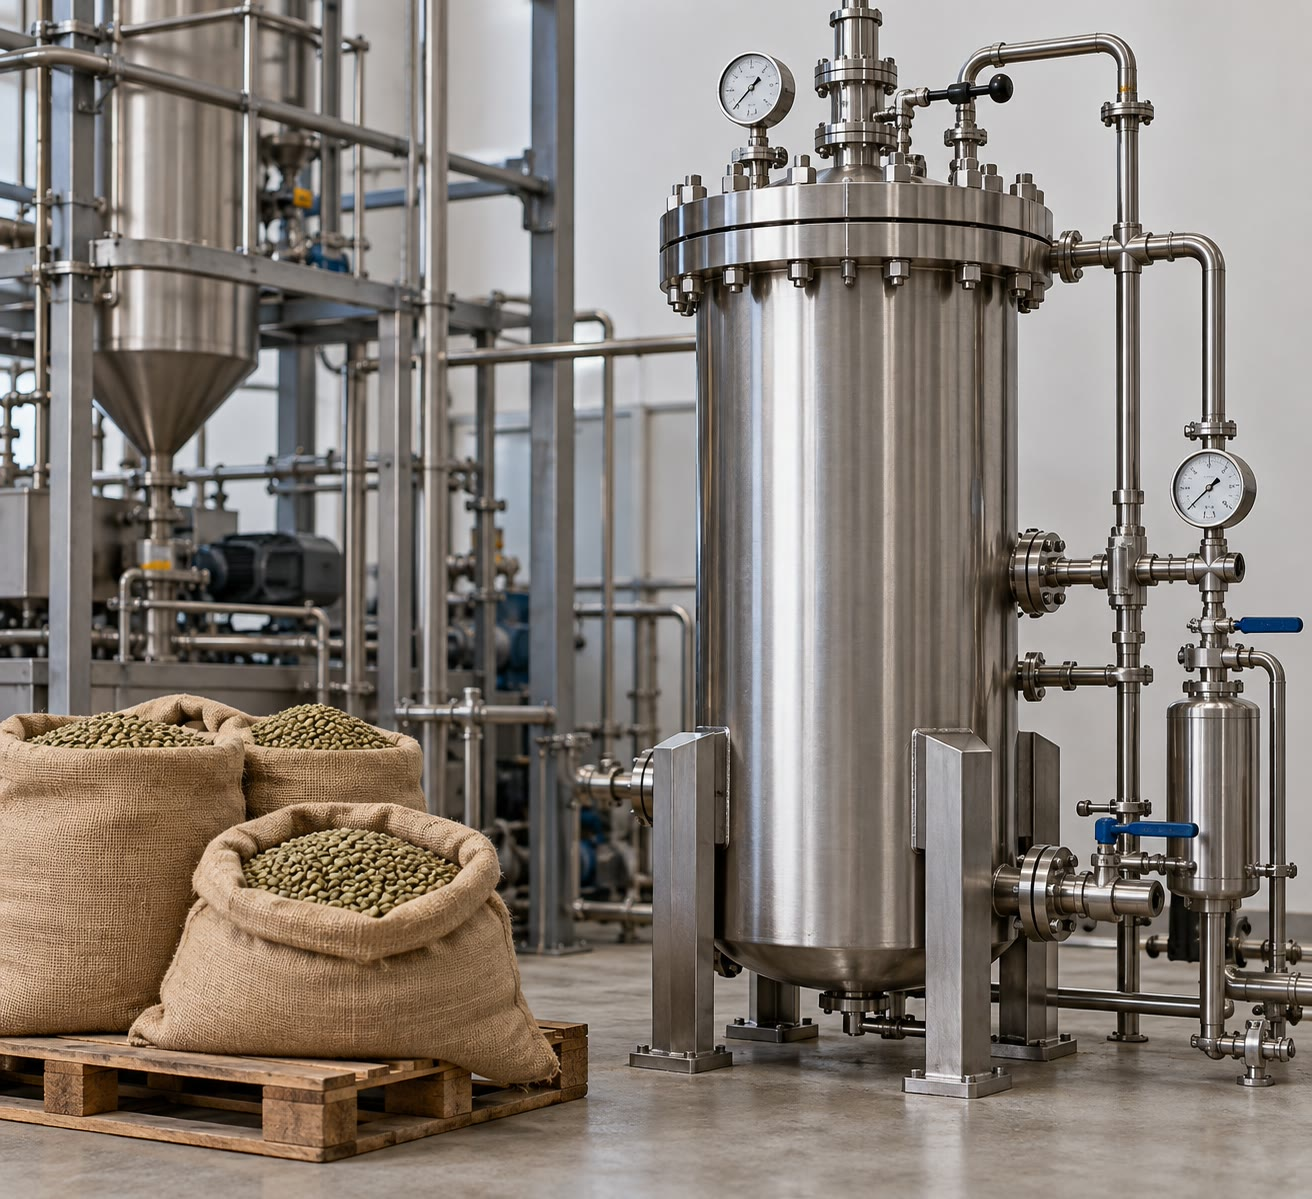
\includegraphics[width=0.45\linewidth,height=6cm,keepaspectratio]{images/book1/ai/g12-scco2-vessel.jpg}

{\small Een hogedrukvat voor \omterm{def:g10:chemical-species:extraction}{extractie}, waarin superkritisch
koolstofdioxide een organisch \omterm{def:g6:solutions-and-solubility:solute}{oplosmiddel} vervangt.}
\end{omfigure}

\section{Oefeningen}

\begin{exercise}[$\star$]\label{exo:g12:synthesis-strategy:1}
Ethanol kan gemaakt worden door hydratatie van etheen,
\ce{C2H4 + H2O -> C2H5OH}, of door vergisting van glucose,
\ce{C6H12O6 -> 2C2H5OH + 2CO2}. Bereken de \omterm{def:g12:synthesis-strategy:atom-economy}{atoomeconomie} van elk.
\end{exercise}

\begin{exercise}[$\star$]\label{exo:g12:synthesis-strategy:2}
Noem in het dipeptideschema van dit hoofdstuk de stap waarin elke
\omterm{def:g12:synthesis-strategy:protecting-group}{beschermende groep} wordt aangebracht, en de stap waarin hij wordt
verwijderd.
\end{exercise}

\begin{exercise}[$\star$]\label{exo:g12:synthesis-strategy:3}
Een fabriek vervangt in een van haar reacties een gechloreerd
\omterm{def:g6:solutions-and-solubility:solute}{oplosmiddel} door water. Welk principe van de \omterm{def:g12:synthesis-strategy:green-chemistry}{groene chemie} past ze toe?
\end{exercise}

\begin{exercise}[$\star$]\label{exo:g12:synthesis-strategy:4}
Waarom verhoogt een overmaat ethanol het \omterm{def:g10:synthesis-yield:yield}{rendement} van een verestering,
maar een \omterm{def:g12:catalysis:catalyst}{katalysator} niet?
\end{exercise}

\begin{exercise}[$\star$]\label{exo:g12:synthesis-strategy:5}
Natriumboorhydride reduceert \omterm{def:g11:functional-groups:carbonyl}{aldehyden} en \omterm{def:g11:functional-groups:carbonyl}{ketonen}, geen \omterm{def:g11:functional-groups:carboxylic-acid}{esters}. Is zijn
reactie met methyl-4-oxopentanoaat (een \omterm{def:g11:functional-groups:carbonyl}{keton} en een \omterm{def:g11:functional-groups:carboxylic-acid}{ester})
\omterm{def:g12:synthesis-strategy:chemoselective}{chemoselectief}? Welke groep verandert?
\end{exercise}

\begin{exercise}[$\star\star$]\label{exo:g12:synthesis-strategy:6}
Eén \omterm{def:g10:the-mole:amount}{mol} ethaanzuur en één \omterm{def:g10:the-mole:amount}{mol} ethanol geven in evenwicht
\qty{0.67}{mol} \omterm{def:g11:functional-groups:carboxylic-acid}{ester}. Stel twee manieren voor om deze hoeveelheid te
verhogen, en één manier om haar sneller te bereiken.
\end{exercise}

\begin{exercise}[$\star\star$]\label{exo:g12:synthesis-strategy:7}
Methyl-4-oxopentanoaat, \ce{CH3-CO-CH2-CH2-CO-O-CH3}, wordt eenmaal
behandeld met natriumboorhydride, en eenmaal met een overmaat
lithiumaluminiumhydride, dat de \omterm{def:g11:functional-groups:carboxylic-acid}{ester} reduceert tot twee \omterm{def:g11:functional-groups:alcohol}{alcoholen}.
Schrijf elk product op.
\end{exercise}

\begin{exercise}[$\star\star$]\label{exo:g12:synthesis-strategy:8}
Welke reacties in het staafdiagram van de atoomeconomieën houden meer dan
drie kwart van de \omterm{def:g7:atoms-and-molecules:atom}{atomen}? Met welke factor is de route in drie stappen
naar ibuprofen beter dan die in zes stappen?
\end{exercise}

\begin{exercise}[$\star\star$]\label{exo:g12:synthesis-strategy:9}
Aspirine wordt gemaakt volgens \ce{C7H6O3 + C4H6O3 -> C9H8O4 + C2H4O2}.
Bereken de \omterm{def:g12:synthesis-strategy:atom-economy}{atoomeconomie} en de massa bijproduct per kilogram aspirine.
\end{exercise}

\begin{exercise}[$\star\star$]\label{exo:g12:synthesis-strategy:10}
Waarom wordt een \omterm{def:g10:synthesis-yield:synthesis}{synthese} onder terugvloeiing verwarmd en niet in een open
kolf? Welke van de twee, snelheid of \omterm{def:g10:synthesis-yield:yield}{rendement}, verbetert het verwarmen?
\end{exercise}

\begin{exercise}[$\star\star$]\label{exo:g12:synthesis-strategy:11}
Tel in de figuur van de twee routes naar ibuprofen de stappen, en zeg
welke principes van de \omterm{def:g12:synthesis-strategy:green-chemistry}{groene chemie} de nieuwere route toepast. Geef er
drie.
\end{exercise}

\begin{exercise}[$\star\star\star$]\label{exo:g12:synthesis-strategy:12}
Een \omterm{def:g10:synthesis-yield:synthesis}{synthese} in drie stappen heeft \omterm{def:g10:synthesis-yield:yield}{rendementen} van \qty{80}{\percent},
\qty{70}{\percent} en \qty{90}{\percent}. Bereken het totale \omterm{def:g10:synthesis-yield:yield}{rendement}.
Welke hoeveelheid uitgangsstof is er nodig om \qty{0.10}{mol}
eindproduct te krijgen, als één \omterm{def:g10:the-mole:amount}{mol} uitgangsstof hoogstens één \omterm{def:g10:the-mole:amount}{mol}
product geeft?
\end{exercise}

\begin{exercise}[$\star\star\star$]\label{exo:g12:synthesis-strategy:13}
Plan de \omterm{def:g10:synthesis-yield:synthesis}{synthese} van het dipeptide Ala--Gly (het zuur van alanine
gebonden aan de \omterm{def:g11:functional-groups:amine}{amine} van glycine): welke groepen bescherm je, en hoeveel
stappen telt het plan?
\end{exercise}

\begin{exercise}[$\star\star\star$]\label{exo:g12:synthesis-strategy:14}
Een bedrijf noemt zijn proces ``groen'' omdat het een \omterm{def:g12:catalysis:catalyst}{katalysator}
gebruikt. Het proces draait bij \qty{250}{\celsius} in benzeen, een giftig
\omterm{def:g6:solutions-and-solubility:solute}{oplosmiddel}, en de \omterm{def:g12:synthesis-strategy:atom-economy}{atoomeconomie} is \qty{35}{\percent}. Beoordeel die
bewering, principe voor principe.
\end{exercise}

\begin{exercise}[$\star\star\star$]\label{exo:g12:synthesis-strategy:15}
Cafeïne wordt uit koffiebonen gehaald met dichloormethaan, een vluchtig
gechloreerd \omterm{def:g6:solutions-and-solubility:solute}{oplosmiddel}, of met superkritisch koolstofdioxide bij
ongeveer \qty{40}{\celsius} en \qty{100}{bar}. Leg uit waarom het tweede
superkritisch is en waarom er een sterk vat voor nodig is, en geef twee
voordelen die het heeft boven het eerste.
\end{exercise}

\section{Probleem: Twee routes naar ibuprofen}

\begin{problem}[{Weekendprobleem --- hoeveel afval vermijdt de route in
drie stappen per ton ibuprofen?}]
\label{pb:g12:synthesis-strategy:1}
% ledger: ibu:boots-ae, ibu:bhc-ae, ibu:boots-steps, ibu:bhc-steps, aw:C, aw:H, aw:O, aw:N, aw:Cl, aw:Na
De oudere route naar ibuprofen \ce{C13H18O2} telt zes stappen. Bij elkaar
opgeteld zijn haar \omterm{def:g7:chemical-reactions:reactant}{beginstoffen} \ce{C10H14}, \ce{C4H6O3},
\ce{C4H7ClO2}, \ce{C2H5ONa}, een zuur dat als \ce{H3O} wordt geteld,
\ce{NH3O} en twee keer \ce{H2O}. De nieuwere route telt drie stappen:
\[
  \ce{C10H14 + C4H6O3 + H2 + CO -> C13H18O2 + C2H4O2} .
\]

\medskip
\noindent\textbf{Deel I --- De vergelijkingen.}
\begin{enumerate}
  \item Controleer dat de vergelijking van de nieuwere route klopt voor
        koolstof, waterstof en zuurstof.
  \item Noem het bijproduct van de nieuwere route.
  \item Welke elementen van de \omterm{def:g7:chemical-reactions:reactant}{beginstoffen} komen bij de oudere route
        helemaal in het afval terecht?
  \item Welke van de twee routes gebruikt \omterm{def:g12:catalysis:catalyst}{katalysatoren}? Welk principe
        past dat toe?
\end{enumerate}

\medskip
\noindent\textbf{Deel II --- Atoomeconomieën.}
\begin{enumerate}[resume]
  \item Bereken de \omterm{def:g10:the-mole:molar-mass}{molaire massa} van ibuprofen.
  \item Bereken de som van de \omterm{def:g10:the-mole:molar-mass}{molaire massa's} van de \omterm{def:g7:chemical-reactions:reactant}{beginstoffen} van de
        oudere route.
  \item Leid daaruit haar \omterm{def:g12:synthesis-strategy:atom-economy}{atoomeconomie} af.
  \item Bereken de som van de \omterm{def:g10:the-mole:molar-mass}{molaire massa's} van de \omterm{def:g7:chemical-reactions:reactant}{beginstoffen} van de
        nieuwere route.
  \item Leid daaruit haar \omterm{def:g12:synthesis-strategy:atom-economy}{atoomeconomie} af.
  \item Wat wordt die als het ethaanzuur als product wordt meegeteld?
\end{enumerate}

\medskip
\noindent\textbf{Deel III --- Afval per ton.}
\begin{enumerate}[resume]
  \item Welke massa \omterm{def:g7:chemical-reactions:reactant}{beginstoffen} wordt er bij de oudere route, bij een
        \omterm{def:g10:synthesis-yield:yield}{rendement} van \qty{100}{\percent}, per ton ibuprofen ingekocht?
  \item Welke massa afval levert die route per ton?
  \item Dezelfde vraag voor de nieuwere route: massa \omterm{def:g7:chemical-reactions:reactant}{beginstoffen} per ton.
  \item Massa ethaanzuur per ton.
  \item Welke massa afval per ton wordt er vermeden als het ethaanzuur als
        afval wordt meegeteld?
\end{enumerate}

\medskip
\noindent\textbf{Deel IV --- \omterm{def:g10:synthesis-yield:yield}{Rendementen} en de echte wereld.}
\begin{enumerate}[resume]
  \item Stel dat elke stap een \omterm{def:g10:synthesis-yield:yield}{rendement} van \qty{90}{\percent} heeft.
        Bereken het totale \omterm{def:g10:synthesis-yield:yield}{rendement} van de oudere route.
  \item Hetzelfde voor de nieuwere route.
  \item Geef, naast de \omterm{def:g8:balanced-equations:equation}{reactievergelijking}, nog een reden waarom minder
        stappen minder afval betekenen.
  \item In de praktijk wordt het ethaanzuur teruggewonnen en gebruikt.
        Welke massa afval per ton levert de nieuwere route dan, bij een
        \omterm{def:g10:synthesis-yield:yield}{rendement} van \qty{100}{\percent}?
  \item Geef het eindantwoord: hoeveel afval vermijdt de route in drie
        stappen per ton ibuprofen?
\end{enumerate}
\end{problem}
